\documentclass{article}
\usepackage{pgfplots}
\pgfplotsset{compat=newest}

\begin{document}

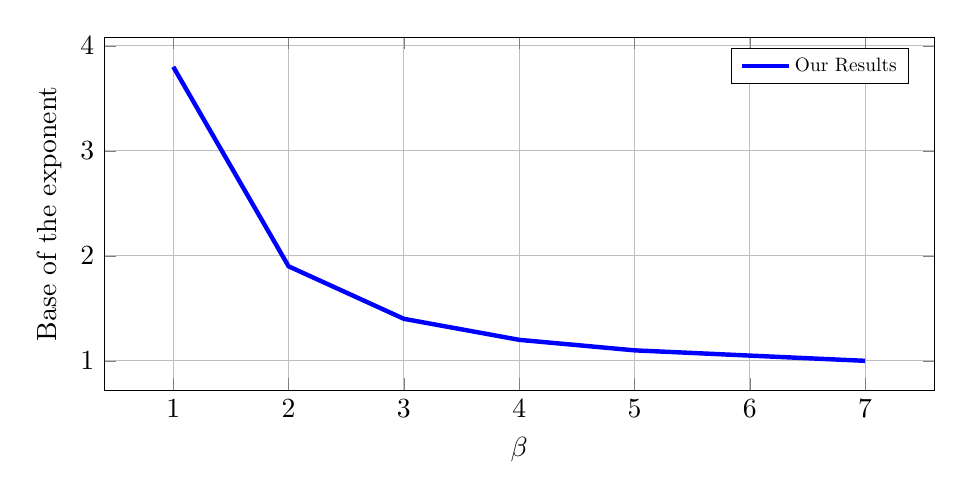
\begin{tikzpicture}
    \begin{axis}[
        xlabel=$\beta$,
        ylabel=Base of the exponent,
        grid=major,
        legend pos=north east,
        width=\textwidth,
        height=0.5\textwidth,
        legend style={nodes={scale=0.7, transform shape}}
    ]
        \addplot[blue, ultra thick] coordinates {(1,3.8) (2,1.9) (3,1.4) (4,1.2) (5,1.1) (6,1.05) (7,1)};
        \legend{Our Results}
    \end{axis}
\end{tikzpicture}

\begin{description}
    \item[A Plot of Running Time] The plot above shows the running time of our algorithm for \texttt{povd}. The \( x \)-axis represents the approximation ratio \(\beta\), and the \( y \)-axis represents the base of the exponent in the running time, which is given by the relationship \( \textnormal{base}^{k} \cdot n^{\Oh(1)} \). Each point \((\beta, d)\) in the plot indicates that the running time of the algorithm for a \(\beta\)-approximation is \( d^{k} \cdot n^{\Oh(1)} \).
\end{description}

\end{document}